\documentclass[conference,a4paper]{IEEEtran}

% Escritura mejorada de fórmulas matemáticas
\usepackage{amsmath}

% Inserción de gráficos
\usepackage{graphicx}

% Escritura de pseudocódigo
\usepackage[kw]{pseudo}

% Escritura mejorada de tablas
\usepackage{booktabs}

% Escritura mejorada de citas bibliográficas
\usepackage{cite}


% Macros traducidas
\def\contentsname{Índice general}
\def\listfigurename{Índice de figuras}
\def\listtablename{Índice de tablas}
\def\refname{Referencias}
\def\indexname{Índice alfabético}
\def\figurename{Fig.}
\def\tablename{TABLA}
\def\partname{Parte}
\def\appendixname{Apéndice}
\def\abstractname{Resumen}
% IEEE specific names
\def\IEEEkeywordsname{Palabras clave}
\def\IEEEproofname{Demostración}


\begin{document}

\title{Título del trabajo (elegir uno original)}

\author{
  \IEEEauthorblockN{Domínguez-Adame Ruiz, Alberto}
  \IEEEauthorblockA{
    \textit{Dpto. Ciencias de la Computación e Inteligencia Artificial}\\
    \textit{Universidad de Sevilla}\\
    Sevilla, España\\
     albdomrui@alum.us.es}
  
  \and
  
  \IEEEauthorblockN{Vilaplana de Trias, Francisco David}
  \IEEEauthorblockA{
    \textit{Dpto. Ciencias de la Computación e Inteligencia Artificial}\\
    \textit{Universidad de Sevilla}\\
    Sevilla, España\\
   fravilde1@alum.us.es}
}

\maketitle


% Resumen
\begin{abstract}
  Escribir aquí dos párrafos indicando el objetivo principal del trabajo, y un
  resumen de las conclusiones obtenidas. Cabe mencionar que este documento se
  ha confeccionado siguiendo el formato de conferencias de IEEE (ver la guía
  para autores para más información, existen plantillas para Word y \LaTeX).
  Este documento se debe emplear como guía, se pueden añadir nuevas secciones
  según sea necesario. Es importante dotarlo de un número razonable de
  referencias bibliográficas.
\end{abstract}


% Palabras claves
\begin{IEEEkeywords}
  Inteligencia Artificial, otras palabras clave…
\end{IEEEkeywords}


\section{Introducción}


Para empezar, el aprendizaje se define como la adquisición del conocimiento de algo por medio del estudio, el ejercicio o la experiencia, en especial de los conocimientos necesarios para aprender algún arte u oficio. Al hablar sobre el aprendizaje automático estaríamos entrando en el campo de la Inteligencia Artificial (IA). Podemos definir esta como un programa de computación diseñado para realizar determinadas operaciones que se consideran propias de la inteligencia humana, como el Aprendizaje Automático (Machine Learning), una rama de la inteligencia artificial, cuyo objetivo es el desarrollo de un sistema (modelo matemático que realiza una determinada tarea)  el cual tiene un mejor desempeño con la experiencia, dados una serie de datos.

Nuestro estudio hace uso de datos relacionales, los cuales están unidos entre sí (tienen una relación) que queda representado como aristas en un grafo, entendiendo un grafo como un conjunto de nodos unido (o no) mediante aristas. En la Fig. \ref{fig:tablaEj} podemos ver un ejemplo de un grafo a partir de unos datos relacionales. 

\begin{figure} % opción de posicionamiento
    \centering
    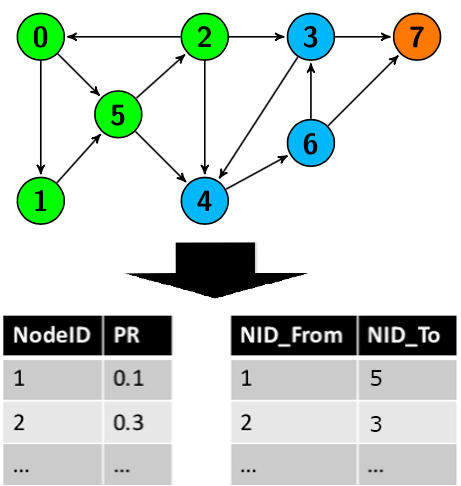
\includegraphics[width=0.4\textwidth]{./ImagenesMemoria/TablaEjemplo}
    \caption{\label{fig:tablaEj}Ejemplo de Grafo}
\end{figure}


Para la realización de este trabajo se ha hecho uso del entorno de desarrollo Jupyter y de la herramienta notebook. El código está escrito mediante el lenguaje de programación Python, usando principalmente las librerías pandas, NetworkX y scikit-learn, y otras como keras, tensorflow y matplot.



Los modelos de clasificación usados son: KNN, Naive Bayes, Árboles de Decisión y Redes Neuronales.

\section{Conjunto de datos y Tarea de predicción a realizar}
]Hemos elegido un dataset ( fíjese en la Figure \ref{fig:dataset}) de la página de streamings en directo twitch.tv , en la que se ve: las visitas, días (ambos de tipo entero) que transmitido un canal en directo, si tiene contrato o no con twitch (partner de tipo Boolean) y si el contenido del canal (id de tipo Integer) es o no para adultos (mature de tipo Boolean). Al ser la propia Twitch la que ofrece este contrato, hemos decidido que la predicción para nuestros modelos sea el atributo partner (true/false). Las aristas (edges) representan si dos usuarios tienen una relación de amistad.

\begin{figure} % opción de posicionamiento
    \centering
    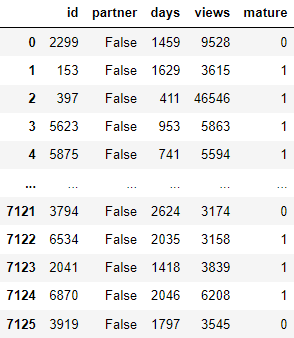
\includegraphics[width=0.3\textwidth]{./ImagenesMemoria/dataset}
    \caption{\label{fig:dataset}Tabla de Datos}
\end{figure}

Este dataset tenía dos tipos de id asociados a cada usuario, uno generado aleatoriamente y otro donde al usuario se le asignaba un valor entre 0 y el numero total de usuarios que recoge el conjunto de datos, por lo que decidimos que eliminar el id generado de forma aleatoria para mayor claridad y sólo hace falta un id por usuario para identificarlos.


Para este estudio hemos decidido que el atributo a predecir será partner. Para ello, haremos uso de los atributos: days, views y mature (el id no es relevante en este caso). Lo hemos planteado como una tarea de clasificación binaria, ya que partner solo tiene dos valores posibles (True o False).

 Por último hemos codificado (codificación one-hot) los valores de mature de Booleano a Integer, pasando True-False a 1-0 respectivamente, para que sea más eficiente estimar las probabilidades del atributo partner.

\section{Métricas Relacionales}
Como este es un trabajo de desarrollo de modelos orientados al aprendizaje automático grafos, hemos elegido una serie de métricas relacionales que aplicaremos como atributos relacionales. En concreto hemos elgido tres métricas:

\begin{enumerate}
\item\textbf{Betweenness centrality}  (Centralidad de intermediación): La centralidad en un grafo puede ser entendida como una medida que determina la relevancia de un nodo dentro del grafo y permite comparar o contrastar dicho vértice con otros. La Betweenness Centrality es una medida de centralidad que cuantifica la frecuencia en la que un nodo se encuentra en el camino más corto entre dos nodos determinados. Cuando en un grafo existen nodos de alta intermediación, estos suelen jugar un rol importante en la estructura a la que pertenecen. Estos nodos también poseen capacidades de ser controladores o reguladores de los flujos de información dentro de la estructura total del grafo. 
\item\textbf{Clustering} (agrupamiento): es una tarea que tiene como finalidad principal lograr el agrupamiento de nodos, para lograr construir subconjuntos de datos conocidos como Clusters.
\item\textbf{Degree} (grado): Número de aristas (relaciones) que inciden sobre el nodo.
\end{enumerate}
 
\section{Algoritmos de Aprendizaje Automático}

\subsection{KNN}

Primero tienes que cargar el archivo de imagen desde su computadora usando el enlace de carga del menú del proyecto. Luego usando el comando 'includegraphics' podrás incluirlo en el documento. Con el entorno de figura y el comando de título podrás agregar un número y un título a la figura. Mira el código de la Figura \ref{fig:tablaEj} en esta sección para ver un ejemplo.



\subsection{Naive Bayes}
% * <stephmigoni@gmail.com> 2018-02-08T19:23:33.559Z:
% 
% Esto es un comentario de prueba
% 
% 

\subsection{Árboles de Decisión}

Usa los comandos table y tabular para iniciar una tabla simple --- mira la tabla~\ref{tab:tabla ejemplo}, como ejemplo. 

\begin{table}
\centering
\begin{tabular}{l c r} 
%nùmero de columnas: 3
l para left & c para centro & r para derecha \\ \hline
Ejemplo & Centrado & Alineado a la\\
Izquierda & 13 & Derecha
\end{tabular}
\caption{\label{tab:tabla ejemplo}Una simple tabla.}
\end{table}



\section{Resultados}

En esta sección se detallarán tanto los experimentos realizados como los
resultados conseguidos:
\begin{itemize}
\item Los experimentos realizados, indicando razonadamente la configuración
  empleada, qué se quiere determinar, y como se ha medido.
\item Los resultados obtenidos en cada experimento, explicando en cada caso lo
  que se ha conseguido.
\item Análisis de los resultados, haciendo comparativas y obteniendo
  conclusiones.
\end{itemize}

Se pueden hacer uso de tablas, como el ejemplo de la tabla~\ref{tab:ejemplo}.

\begin{table}
  \caption{Ejemplo de tabla}
  \label{tab:ejemplo}
  \centering
  \begin{tabular}{ccc}
    \toprule
    A & B & C \\
    \midrule
    1 & 2 & 3 \\
    4 & 5 & 6 \\
    \bottomrule
  \end{tabular}
\end{table}


\section{Conclusiones}

Finalmente, se dedica la última sección para indicar las conclusiones obtenidas
del trabajo. Se puede dedicar un párrafo para realizar un resumen sucinto del
trabajo, con los experimentos y resultados. Seguidamente, uno o dos párrafos
con conclusiones. Se suele dedicar un párrafo final con ideas de mejora y
trabajo futuro.


\section{Bibliografía}
\begin{thebibliography}{00}
\bibitem{b1} G. Eason, B. Noble, and I. N. Sneddon, ``On certain integrals of Lipschitz-Hankel type involving products of Bessel functions,'' Phil. Trans. Roy. Soc. London, vol. A247, pp. 529--551, April 1955.
\bibitem{b2} J. Clerk Maxwell, A Treatise on Electricity and Magnetism, 3rd ed., vol. 2. Oxford: Clarendon, 1892, pp.68--73.
\bibitem{b3} I. S. Jacobs and C. P. Bean, ``Fine particles, thin films and exchange anisotropy,'' in Magnetism, vol. III, G. T. Rado and H. Suhl, Eds. New York: Academic, 1963, pp. 271--350.
\bibitem{b4} K. Elissa, ``Title of paper if known,'' unpublished.
\bibitem{b5} R. Nicole, ``Title of paper with only first word capitalized,'' J. Name Stand. Abbrev., in press.
\bibitem{b6} Y. Yorozu, M. Hirano, K. Oka, and Y. Tagawa, ``Electron spectroscopy studies on magneto-optical media and plastic substrate interface,'' IEEE Transl. J. Magn. Japan, vol. 2, pp. 740--741, August 1987 [Digests 9th Annual Conf. Magnetics Japan, p. 301, 1982].
\bibitem{b7} M. Young, The Technical Writer's Handbook. Mill Valley, CA: University Science, 1989.
\end{thebibliography}


\end{document}
